\documentclass[15pt,a4paper]{article}

\usepackage{amssymb}
\usepackage{vmargin}
\usepackage{csquotes}
\usepackage{graphicx}
\setmargins{2.5cm}{1.5cm}{16.5cm}{23.42cm}{10pt}{1cm}{0pt}{2cm}
\graphicspath{ {.} }

\title{Informe Final. Clash Royale\\ Ingeniería de Software + Base de Datos.}
\author{Karen Dianelis Cantero Lopez. C311 \\ Luis Alejandro Rodriguez Otero C311\\  Hector Miguel Rodriguez Sosa C311 \\ Sebastian Suarez Gomez C311 }
\date{}

\begin{document}

\maketitle

\section{Introducción}
El producto tiene como objetivo analizar los datos de los usuarios de Clash Royale y 
proporcionar la información más relevante sobre su comportamiento, patrones de juego, 
estrategias y rendimiento. Se utilizan análisis de métricas de participación y evaluación 
de la experiencia del usuario.
En el presente informe se describe el proyecto. Se presentan los requerimientos 
específicos funcionales, no funcionales y del entorno. Las funcionalidades del producto
se muestran a partir de un modelo de casos. En la arquitectura del proyecto se presentan 
la arquitectura general y la arquitectura de diseño del backend. En el modelo de datos se 
muestra el modelo de base de datos. Estos y otros aspectos significativos para la 
realización del producto se abordan a continuación. 



\section{Requerimientos Específicos}
\subsection*{Requisitos Funcionales}
\begin{enumerate}
\item El usuario puede registrarse e iniciar sesión.
\item El usuario puede visualizar gráficamente la popularidad del juego; es decir, puede 
ver gráficamente la cantidad de batallas y desafíos en el año. 
\item Realizar batallas entre jugadores simulando el resultado.
 Visualizar las cartas con sus características.
\item Realizar operaciones CRUD sobre las entidades.
\item Realizar consultas a la base de datos y exportar los resultados de dichas consultas 
en archivos .pdf o .csv.
\item Realizar un análisis del mazo del jugador.
\item Realizar análisis de métricas de participación: el sistema es capaz de analizar y 
proporcionar información detallada sobre la participación de los usuarios en el 
juego. 
\end{enumerate}

\subsection*{Requisitos No Funcionales}

\begin{enumerate}
\item Seguridad: El sistema garantiza la confidencialidad, integridad y autenticación de 
los datos de los usuarios. El acceso a la plataforma es controlado por nombre de 
usuario y contraseña. Una vez el usuario esté autenticado en la plataforma, se le 
asignará un token jwt. En caso de este expirar luego de haberse iniciado sesión, 
se necesitará que se autentique de nuevo. 
\item  Rendimiento: El sistema es eficiente y tiene un rendimiento óptimo. Asegura 
tiempos de respuesta rápidos y capacidad para manejar el volumen de datos y
usuarios sin degradar la calidad del servicio. 
\item Usabilidad: La interfaz del sistema es intuitiva, fácil de usar. Se siguen las mejores 
prácticas de diseño de experiencia de usuario (UX) para garantizar una interacción 
fluida y positiva. 
\item El sistema alacena todos los datos en una base de datos SQL Server. A través del 
sistema se pueden realizar consultas requeridas y algunas parametrizadas. 
\item El sistema cuenta con un apartado FAQ donde se le darán respuesta a algunas 
preguntas técnicas que puedan tener los usuarios.
\item Disponibilidad: Existen tres tipos de usuarios (user, admin y superadmin), donde 
a cada uno se le garantiza el acceso a un determinado tipo de información.
\item Diseño e implementación: En el proyecto se emplea una arquitectura monolítica. 
Para la construcción del Backend, se usó .NET Core con C\# y para el Frontend, 
se usó Angular. En el Backend, se usó una arquitectura de diseño basada en un 
dominio conocida como DDD. Para el trabajo con la base de datos se usó Entity 
Framework Core.
\end{enumerate}

\subsection*{Requisitos de entorno}
\begin{enumerate}
\item Framework: .NET Core 7 y Angular.
\item Lenguaje de programación: C\# y Typescript.
\end{enumerate}


\section{Funcionalidades del producto}
Modelo de casos


\begin{center}
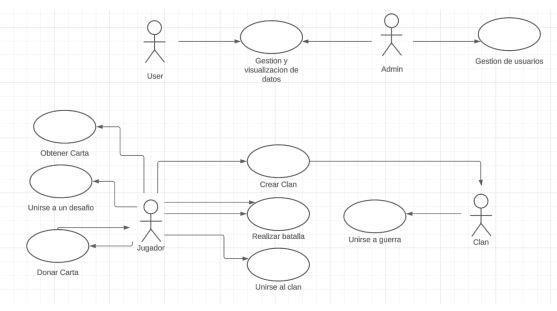
\includegraphics[width=0.8\textwidth]{casos}
\end{center}

\section{Enfoque Metodológico}
Para la creación, se dividió el proyecto teniendo en cuenta las destrezas de los individuos 
y cada uno trabajó en un sector específico. El jefe de equipo repartió las tareas basándose 
en lo anterior. 

\section{Arquitectura}
En el proyecto en general, se utiliza una arquitectura monolítica donde lo componentes 
se integran en una sola unidad y son compatibles entre sí.

\subsection*{Diseño de Backend}
\begin{center}
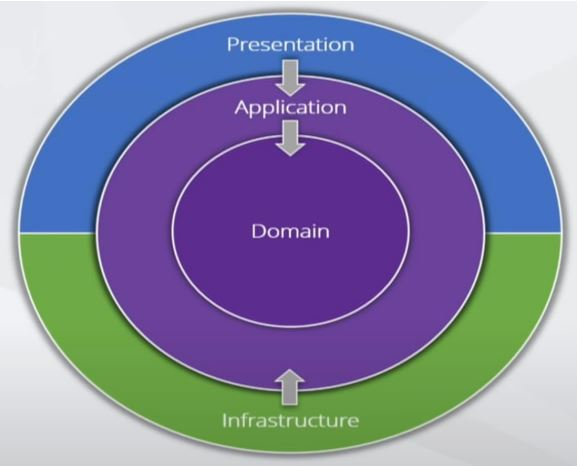
\includegraphics[width=0.8\textwidth]{back}
\end{center}


Se escogió esta arquitectura de diseño para tener el proyecto correctamente separado y 
garantizar las mejores prácticas de programación. Se emplea el patrón de diseño CQRS, 
donde se separan las responsabilidades en commands y queries.
\begin{enumerate}
\item Domain: Entidades, excepciones, errores y posibles partes que no necesiten de ninguna 
otra capa.
\item Application: Interfaces y posibles objetos que interactúen con el Domain.
\item Infrastructure: Diferentes implementaciones de las interfaces de repositorio y todo lo 
relacionado con la base de datos.
\end{enumerate}

\section{Patrones de Visualización}
Una gráfica de líneas muestra la popularidad del juego por mes (cantidad de batallas en 
el año). Mientras el proyecto avance se irán agregando más formas de visualización de 
datos.

\section{Modelo de Datos}
Base de datos:
\begin{center}
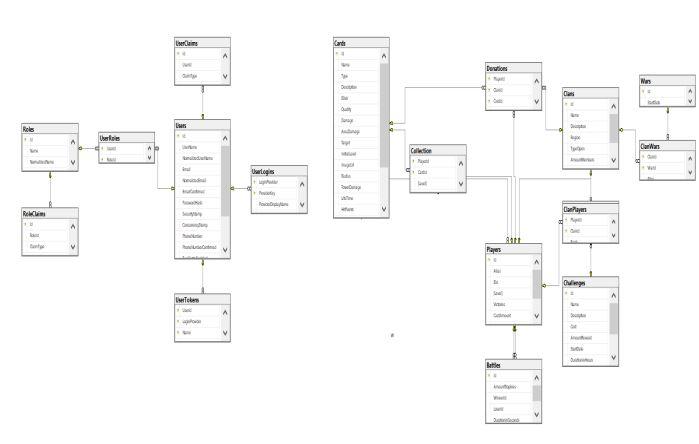
\includegraphics[width=0.8\textwidth]{bd}
\end{center}




\end{document}